\documentclass[border=10pt]{standalone}
\usepackage{pgfplots}
\pgfplotsset{compat=1.18}
\begin{document}
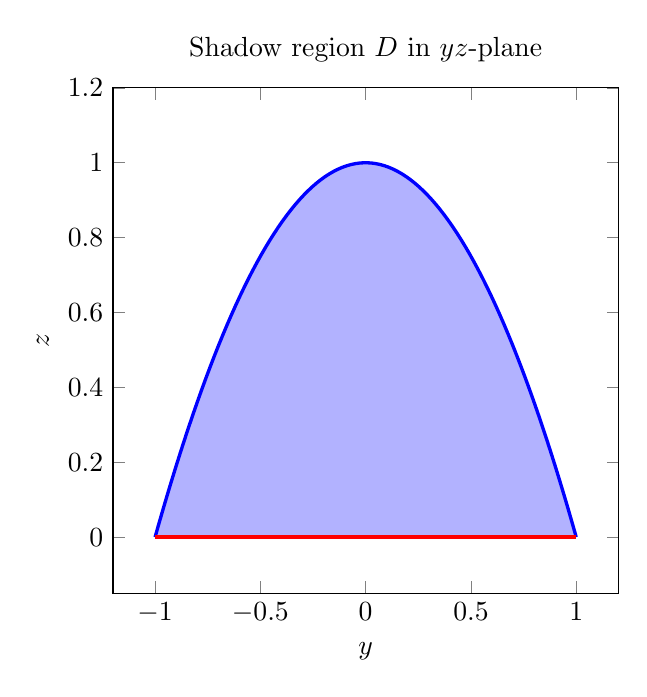
\begin{tikzpicture}
\begin{axis}[
    width=8cm, height=8cm,
    xlabel={$y$}, ylabel={$z$},
    xmin=-1.2, xmax=1.2, ymin=-0.15, ymax=1.2,
    title={Shadow region $D$ in $yz$-plane},
    axis on top]
% shaded region 0 <= z <= 1-y^2
\addplot[domain=-1:1, samples=100, draw=none, fill=blue!30] {1-x^2} \closedcycle;
% curve z = 1 - y^2
\addplot[domain=-1:1, samples=100, very thick, blue] {1-x^2};
% line z = 0
\addplot[domain=-1:1, samples=2, very thick, red] {0};
\end{axis}
\end{tikzpicture}
\end{document}